% !TEX root=/home/tavant/these/manuscript/src/manuscript.tex

\section{Study of the radial electron heating}
\label{sec-rheating}
    We have seen in \cref{fig-boeuf-temporal,fig-boeuf_axialtwo} that the radial electron temperature is constant in both time and space, leading to a large anisotropy.
    This could be due to the lack of collision in the test-case of Boeuf.
    Thus, we investigate thereafter the impact of the neutrals on the electron anisotropy by modeling the collisions with the \ac{MCC} algorithm.
    
  \subsection{Boeuf test-case with collisions} \label{subsec-MCC_boeuf}
    % Script on Juno (CH-6_Boeuf)

    To model the neutral density, we inject at the anode a constant xenon flow of rate $\dot{m} = 5 \milli\gram\per\second$ at a temperature of $T_g = 640\,\kelvin$.
    Using a typical surface area, this corresponds to a neutral density at the anode of $n_g=3.0 \times 10^{19}$ {m}$^{-3}$ and a mean velocity of $u_g = 200 \,\meter\per\second$.
    
    The evolution of the neutral density is model using the system of \ac{1D} fluid equations, as we neglect the evolution in the azimuthal direction\string:
    \begin{equation}
    \left\{
    \begin{gathered}
    \partial_{t} n_g + \partial_{z}(n_g u_g) = - S_{iz}\\
    \partial_{t}(n_g u_g) + \partial_{z}(n_g u_g^{2}) = -\partial_{z}p_g - S_{iz} u_g \\
    \partial_{t}E + \partial_{z}(Eu_g) = - \partial_{z}(p_g u_g)
    \end{gathered}
    \right.
    \label{eq-euler}
    \end{equation}
    with $u_g, p_g$ the neutral axial velocity and the pressure, respectively, $S_{iz}$ is the imposed ionization source term, and $E$ the energy per volume unit
    \begin{equation}
      E =  \frac{p_g}{\gamma - 1} + \frac{1}{2} n_g u_g^{2},
    \end{equation}
    with $\gamma=5/3$.
    This Euler system is solved using the HLLC Riemann solver, which as been validated on the  shock tube test case.
    For sake of simplicity, the neutral temperature is kept constant by adding an artificial source term in the third equation of \cref{eq-euler}
    \begin{equation} \label{eq-artificial}
      S_3 = -\frac{1}{\tau} \lp  \frac{p_g}{\gamma - 1} - \frac{n_g R T_0}{\gamma-1} \rp
    \end{equation}
    with $T_0$ the desired temperature, and $\tau$ the "thermalization time" to reach $T_0$.
    We chose $\tau$ small enough so that $T_n$ does not vary much, while preserving the Courant-Friedrich-Levy condition.
    In practice, we use $\tau = 10\,\nano\second$.
    
    Finally, the neutral density is used in the \ac{MCC} algorithm to model the electron-neutral and ion-neutral scattering and momentum transfer, but the creation of particles remains imposed by the same ionization profile $S_iz$ as in \cref{sec-Zthetaresults}.
    \Cref{fig-boeuf-neutrals} shows the neutral density and velocity obtained at steady-state.

    \begin{figure}[hbt]
      \centering
      \begin{tabular}{cc}
        \subfigure{boeuf_MCC_ng}{a}{20,15} &
        \subfigure{boeuf_MCC_vg}{b}{20,15} \\
      \end{tabular}
      \caption{Axial profile at steady-state ($t=10\,\micro\second$) of ({\bf a}) the neutral density and  ({\bf b})  the neutral axial velocity, for  simulation with the electron-neutral scattering. }
      \label{fig-boeuf-neutrals}
    \end{figure}

    We see in \cref{fig-boeuf-neutrals} that the neutral density is depleted between the anode and the cathode because of the ionization.
    The neutral density gradient and the ionization accelerates the neutrals in the axial direction by a factor of two, which reduces even more the neutral density.
    Thus, the impact of the neutral collisions will be more significant close to the anode.

    \begin{figure}[hbt]
      \centering
      \begin{tabular}{cc}
        \subfigure{boeuf_mean_Te}{a}{20,20} &
        \subfigure{boeuf_mean_Tez_profile_MCC}{b}{20,15} \\
      \end{tabular}
      \caption{({\bf a}) temporal evolution of the electron kinetic energy in the three directions and  ({\bf b}) axial profile of the electron temperature at steady state obtained for the simulation case of Boeuf with the electron-neutral scattering. }
      \label{fig-boeuf-temporalMCC}
    \end{figure}
    
    \Cref{fig-boeuf-temporalMCC} shows the temporal evolution of the mean electron kinetic energy on the left, and on the right it shows the axial profile of the electron temperatures, decomposed in the three directions.\footnote{The kinetic energy is the sum of the temperature and the kinetic energy of the drift velocity}
    We see that they is a small transfer of energy between the radial direction and the others.
    In particular, close to the anode where the gas density is high, the radial and axial temperatures decrease below the initial temperature $\Te_{, inj}=5\,\volt$.
    In contrast, at the maximum of the magnetic field where the axial and azimuthal electron temperatures are the highest, the radial electron temperature increases to $\Te_R=7\,\volt$.
    However, the anisotropy stays significant, compared to the observation of the radial-azimuthal simulations presented in \cref{ch-2}.
    Therefore, the neutral density is not the main reason for the electron heating.


    \subsection{Radial Joule electron heating } \label{subsec-radial-heating}
  
  The large anisotropy observed in \Cref{fig-boeuf-temporal,fig-boeuf-temporalMCC}, compared to the results of \cref{ch-2} does not come from the electron-neutral scattering.
  Thus in this section, we investigate the electron energy gain due to Joule heating
  \begin{equation} \label{eq-epower}
      \vect{P_{\rm J}} = \vect{J_e} \cdot \vect{E},
  \end{equation}
  with $\vect{J_e}$ the electron density current and $\vect{E}$ the electric field.
  \Cref{fig-epower_radialone} shows the radial profiles of the electron (and ion) current density $< J_{e, R}>$ and the radial electric field $ < E_R >$, averaged in the azimuthal direction.
  We observe that the ion and electron current densities are equal to each-other, and they increase linearly with the radial position.
  This was expected, as we use a uniform artificial injection of particles, which compensates the radial losses (see \cref{sec-bidimentionnal_simulation} for more details).

  \begin{figure}[hbt]
    \centering
    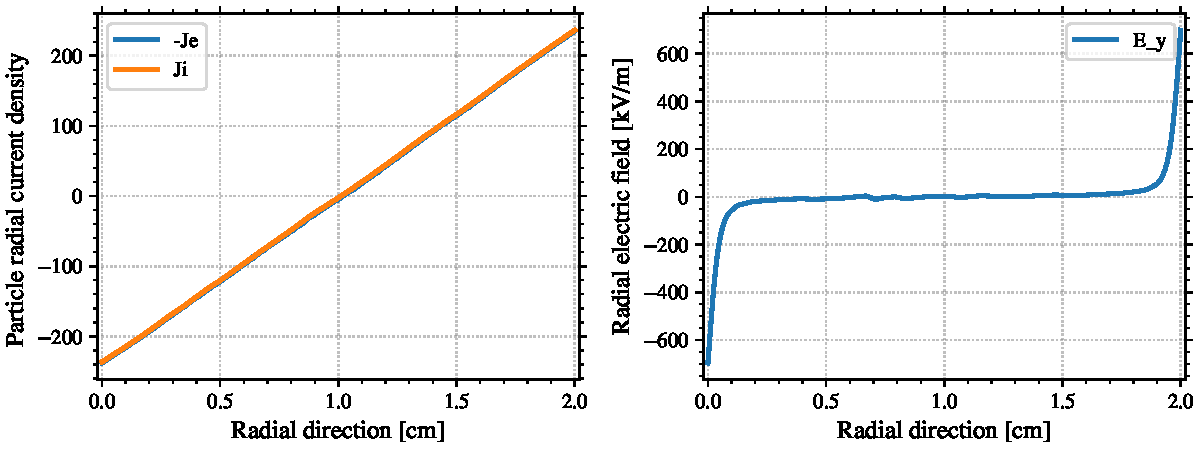
\includegraphics[width=\textwidth]{R_joule_heating_one}
    \caption{Radial profiles averaged in the azimuthal direction of (left) the electron and ion current densities and (right) radial electric field in the radial-azimuthal \acs{PIC} simulation presented in \cref{ch-2}. }
    \label{fig-epower_radialone}
  \end{figure}
  
  The radial electric field $E_r$ seen in \cref{fig-epower_radialone} is very small in the center of the system, and increases drastically in the sheath close to the walls.
  Consequently, from the product $< J_{e, R}>  < E_R >$ we could expect that the radial Joule electron heating to be small in the center of the discharge, and negative in the sheath.
  \Cref{fig-epower_radial} shows the mean Joule heating in the radial direction ${P_{\rm J, R}} = < J_{e, R} E_R >$ measured in the \ac{PIC} radial-azimuthal simulation, and the product of the mean quantities $< J_{e, R}>  < E_R >$.

  \begin{figure}[hbt]
    \centering
    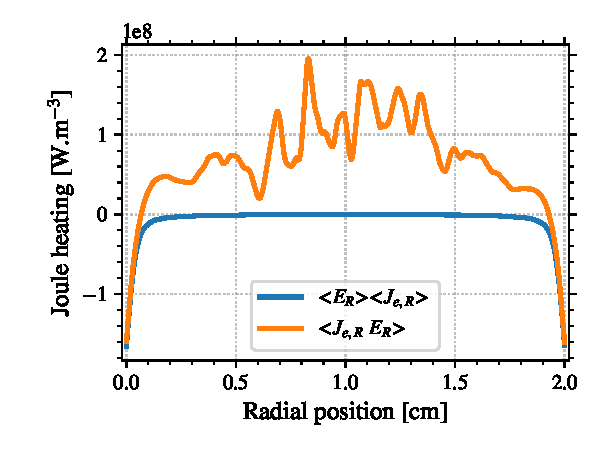
\includegraphics[width=\defaultwidth]{R_joule_heating_two}
    \caption{Electron power gain in the Radial-azimuthal }
    \label{fig-epower_radial}
  \end{figure}

  We see in \Cref{fig-epower_radial} that, unexpectedly,  the mean Joule heating $\bar{P_{\rm J, R}}$ is not zero in the center of the simulation.
  This means that there is an energy transfer to the radial direction of the electrons due to the correlation between the fluctuations of $\vect{J_e}$ and $\vect{E}$.
  Consequently, for this energy transfer to be self-consistently observe in a simulation, the radial direction needs to be resolved.

  A similar radial heating has been observed by \citet{heron2013}.
  The authors observe no heating when the instability was only perpendicular to the magnetic field, as it is in a \ac{1D} or a \ac{2D} axial-azimuthal simulation.
  However, when the direction parallel to the magnetic field is resolved, the electrons are heated.
  However, the physical mechanism remains unclear.
  In \citet{janhunen}, the authors observe a similar radial heating of the electrons, but due to the presence of a \ac{MTSI}.
  As discussed in the previous chapters, we do not observe the \ac{MTSI} in our simulations, meaning that it has to be due to another mechanism.




\section{Conclusion on the 2D PIC axial-azimuthal simulations}

In this chapter, we have investigated the impact of the radial direction in a \ac{PIC} simulation that simulates the axial and azimuthal directions.
We proposed an algorithm in order to introduce in a \ac{2D} azimuthal-axial simulation the effects of the radial direction.
More precisely, we modeled the losses of particles, corresponding to fully absorbing walls without secondary electron emission.
The model imposes a pseudo-local flux neutrality at the wall, reproducing the effect of a floating sheath.
We followed the test-case proposed by \citet{boeuf2018}.
It uses a forced ionization source term, which removes the breathing mode.
The breathing mode is an ionization instability that makes the analyzing of the simulations more complex.

The model of radial loss has successfully shown its ability to reduce the plasma density and electron temperature.
We were able the obtain a steady-state for three cases\string: one without radial losses, and two with losses using a radial length $L_R=4\,\centi\meter$ and $L_R=2\,\centi\meter$.
We observe that the radial losses reduce the electron density slightly and that the axial electric field is almost not affected.
On the other hand, the electron temperature is significantly reduced and not only in the radial direction but in the three directions.
The reduction of the electron temperature is correlated to a substantial diminution of the electron axial mobility.

As the simulations are collisionless, the electron mobility comes from the azimuthal instability.
We observed that the amplitude of the instability, thus the induced electron axial mobility, is reduced by the radial losses.
Several hypotheses that could explain the diminution of the wave amplitude have been discussed.
The most probable reasons are the diminution of the electron azimuthal drift, hence the reduction of the growth rate, and the fact that the radial losses absorb the particles preferentially at the maximum of the oscillations.

The reduced wave amplitude is related with a decreasing of the ion-wave trapping, which seems to be one of the dominant mechanism of saturation when the radial losses are not modeled.
In addition, the characteristics of the wave (frequency, wavelength) are modified.
More precisely, in the upstream region, close to the maximum of the magnetic field, the waves are not affected.
On the other hand,  in the downstream region, a low-frequency and large wavelength oscillation is present when no radial losses are modeled.
The amplitude of this large wave is reduced for $L_R=4\,\centi\meter$, and disappears for $L_R=2\,\centi\meter$.
We believe that this large wavelength oscillation comes from a nonlinear inverse cascade mechanism, most certainly related to the ion-wave trapping.
As the wave amplitude is smaller, the nonlinear stage of the wave is not reached when the radial losses are modeled.


\vspace{1em}
Lastly, we observed that the electrons are less isotropic than seen in the radial-azimuthal simulation, even in the presence of electron-neutral scattering.
We noted that in the radial-azimuthal simulation, where the radial electric field is self-consistently computed, the mean radial electron Joule heating is important in the plasma bulk.
This radial heating seems to be due to the instability, that presents radial structures.
This joule heating is absent of the \ac{2D} axial-azimuthal simulation.
Therefore, a better understanding of the radial heating of the electrons is necessary, so that low-dimensional fluid and \ac{PIC} simulation can realistically model the plasma-wall interactions.
The electron distribution function measured in experiments or observed in a \ac{3D} \ac{PIC} simulation would be beneficial to give to the community insights on the coupling and the relative importance of the radial, axial and azimuthal directions.

